% =====================================================================
%  USER STUDY + FINDINGS  --  P1-P13
%
%  Replaces the 2 Aug 2026 preliminary section (findings.tex), which
%  reported interviews from P1-P3 only, trajectories from P1-P7, and
%  world building from P1-P10.  Every number below is recomputed at
%  P1-P13 scope and was verified against the source data on 3 Sep 2026:
%    - telemetry  : SessionLogs/_analysis_all/*.csv
%    - worlds     : SessionLogs/P*/scenario/*/scene.json
%    - interviews : full semantic coding + affinity map over P1-P13
%
%  Requires: graphicx, booktabs.  Uses figure*/table* (two-column class).
%  Figures: figures_p1p13/ (regenerated at P1-P13 scope).
% =====================================================================

\section{User Study}
\label{sec:study}

\subsection{Design and protocol}
\label{sec:study:design}

Thirteen participants (P1--P13) completed sessions of 49--82 minutes.
Each participant experienced the same four sidewalk scenarios --- a
head-on \emph{narrow road}, a blind \emph{corner}, a \emph{crossroad}
crossing, and an exit \emph{out of a store} --- twice: once embodying a
wheelchair-using pedestrian, and once driving the delivery robot. Each
pair was followed by a think-aloud review in which participant and
researcher replayed the logged trial together, and each scenario closed
with a world-building pass in which the participant rebuilt the scene
to make it harder. Scenario order varied between participants, so
themes are aligned by scenario type rather than by position, and
scenario-level ratings are treated as ordinal. P11's session was
conducted in Mandarin; quotations from it are translated.

Three data streams contribute to the findings.
\emph{(i)~Interviews.} All thirteen sessions were transcribed and
semantically coded, then affinity-mapped into the frame, strategy,
signalling, world-building and deployment code families cited
throughout below.
\emph{(ii)~Trajectories.} Positions are logged at 10\,Hz for the robot,
the wheelchair agent and the scripted background pedestrian. The
corpus comprises 204 robot runs --- 74 under the autonomous planner, 69
under joystick teleoperation, 36 executing a route the participant drew
before the trial, 22 re-runs after the participant had edited the
world, and 3 plain re-runs --- together with the 74 paired
pedestrian-seat trials in which the participant drove the wheelchair
while the planner drove the robot.
\emph{(iii)~World building.} 143 objects placed across 39 edited worlds
(13 participants $\times$ up to four scenes).

Because the design is within-participant, quantitative comparisons are
per-participant contrasts; we report them descriptively, to establish
that a direction is consistent rather than to estimate an effect size.

% ---------------------------------------------------------------------
\subsection{How the robot's presence is perceived and evaluated}
\label{sec:study:rq1}

\textbf{The ratings disagree, and the telemetry shows the disagreement
is real rather than noise.} The two largest variances in the session
rating sheet are the blind corner on comfort ($\sigma^2 = 7.81$) and
the narrow road on path adjustment ($\sigma^2 = 7.21$). The corner is a
shrug for some participants (P7 and P10 both rated comfort 9) and the
worst moment of the study for others (P6 rated comfort 2 with path
adjustment 10). The trial telemetry reproduces the split as behaviour
instead of averaging it away. Across the 74 pedestrian-seat trials,
\textbf{96\%} (71/74) contain at least one full stop. On the narrow
road, where the encounter is head-on, the median participant drops to
\textbf{0.40$\times$} their own free-walking speed at closest approach
and stops 4.4 times per trial, spending a median of 3.0\,s stopped
($n=14$). The corner is bimodal exactly as its variance predicts: the
median trial shows no slowdown at all (1.00$\times$), yet 41\% of
trials brake below 0.7$\times$ ($n=17$).

\textbf{Two response styles account for the split.} Some participants
absorbed the encounter by giving up ground they would not normally give
up, and rated it as high disruption and low comfort. P6 stepped onto
the hatchway \emph{on purpose} to escape the robot --- ``it was coming
too fast that I couldn't go around'' --- and scored comfort 2 with
adjustment 10. P9 named the trade as she made it: ``if I need to get to
my destination now, I'm more likely to step on something I wouldn't
normally step on,'' and, asked whether ceding the path frustrated her:
``Probably. \textbf{Only because it's not human}.'' Others walked on
and were fine. P12 proceeded confidently because ``this kind of robot
has a camera'' --- then admitted she watched it anyway, because
software fails: ``maybe they cannot recognize the stuff in front of
them\dots\ I was a little worried about whether the robot successfully
detected me.'' The same encounter, two different priors about the
robot.

\textbf{Disruption and comfort come apart as evaluations.} Several
participants were comfortable precisely because being blocked did not
signify. P7 adjusted ``only slightly --- just as much as I would
another person'' and rated comfort 10 (``that's how people walk too'');
P4 rated her own adjustment 8 yet called it ``not cumbersome''; P12
rated adjustment 8 and shrugged --- ``that also happens if a human is
coming.'' The reverse case exists too: P5 adjusted her path
\emph{zero} at the crossroad and still rated comfort 4 --- ``it's still
in your line of sight, so you also have to be cautious of it'' --- a
vigilance tax with no detour attached.

\textbf{What participants actually did was pre-emptively clear out of
the robot's way, because they did not trust it to react.} P4: ``I
wanted to avoid the robot, to get out of its path, \emph{as opposed to
having it recognize me and move}.'' P12: ``I try to avoid the robot
instead of waiting for the robot to avoid me.'' P6: ``I'm gonna move
over, because I don't trust it enough to not hit me.'' On the
think-aloud, most of the disturbance turns out to come not from having
to yield --- participants yield to people all day, and several said so
--- but from what sits underneath the yield: the \emph{uncertainty}
that forces the hesitation (P8, stuck behind the slow robot: ``I can't
predict where it's actually gonna go''), the \emph{unreadable
capability} that makes unilateral avoidance the only safe move (P13: a
person is ``probably as agile as I am\dots\ with the robot, I'm not
sure how smart it is or how it's gonna move''), and the specific sting
of conceding space to a machine (P9's ``only because it's not human'').

\textbf{The frame participants borrow predicts their entire ruleset.}
Most reached for an existing schema: a vehicle (P1's ``mini car,'' P3's
``little baby car''), a pet (P9's ``dog off the leash\dots\ better,
because it can't fight me''), another pedestrian (P7, P12), or a cute
curiosity (P10, P13 --- a frame that buys goodwill but invites
interference; P13 abandoned her walk entirely to look at the robot's
face). P7, holding the pedestrian frame, rated every scenario as no
worse than a human doing the same thing; P9, holding the pet frame,
forgave confusion but wanted supervision; the vehicle framers imported
traffic norms wholesale.

\textbf{Evaluations move with experience, which is what makes the
simulator an instrument rather than a survey.} P5 took the efficient
shortcut as the robot and recanted it within a minute; P13 steered
around a stopped woman, then judged herself on the replay --- ``now
thinking back, it was a little bit rude''; P9 switched into the robot's
first-person camera (``this is much scarier\dots\ looking at people's
knees'') and drove differently for the rest of her session.

\textbf{Behaviour editing isolates the variable, and the variable is
predictability, not proximity.} The crossroad carries the cleanest
manipulations, because the scene and the agents stay fixed and only
speed or heading is edited. P11's comfort collapsed from 8 to 3--4 when
the robot crossed faster and diagonally (``it squeezed me off the edge
--- why is this robot trying to take the road from me?''); P13's
version made her ``jump a little to avoid it''; P4 tolerated the same
speed-up (``I just stopped, let it pass\dots\ a little whoa''); P12
normalised it outright. The control edit ran the other way: with the
pedestrian forced onto a known straight path, P3's whole problem
dissolved --- ``way more relaxed\dots\ you do what you gotta do, and
I'll do what I gotta do.''

% ---------------------------------------------------------------------
\subsection{What socially compliant behaviour participants prefer}
\label{sec:study:rq2}

\begin{table}[t]
  \centering
  \small
  \setlength{\tabcolsep}{4pt}
  \caption{The preference ladder. Robot runs at P1--P13, comparing what
  the planner does, what participants drove, and what they drew as the
  ideal. Every measure moves monotonically along the ladder. Trailing
  idle at the goal is excluded from all stop measures; the speed ratio
  is the ratio of mean speed near a human to mean free speed.}
  \label{tab:ladder}
  \begin{tabular}{lrrr}
    \toprule
     & \textbf{auto} & \textbf{driven} & \textbf{drawn}\\
     & planner & by participant & by participant\\
     & ($n{=}74$) & ($n{=}69$) & ($n{=}36$)\\
    \midrule
    Stops $\geq$1\,s near a human   & 0.00 & 0.67 & 0.83\\
    Time stopped $\geq$1\,s (s)     & 0.2  & 4.5  & 7.2\\
    Speed near humans $\div$ free   & 0.93 & 0.83 & 0.77\\
    Path efficiency (median)        & 0.99 & 0.94 & 0.90\\
    \bottomrule
  \end{tabular}
\end{table}

\begin{figure}[t]
  \centering
  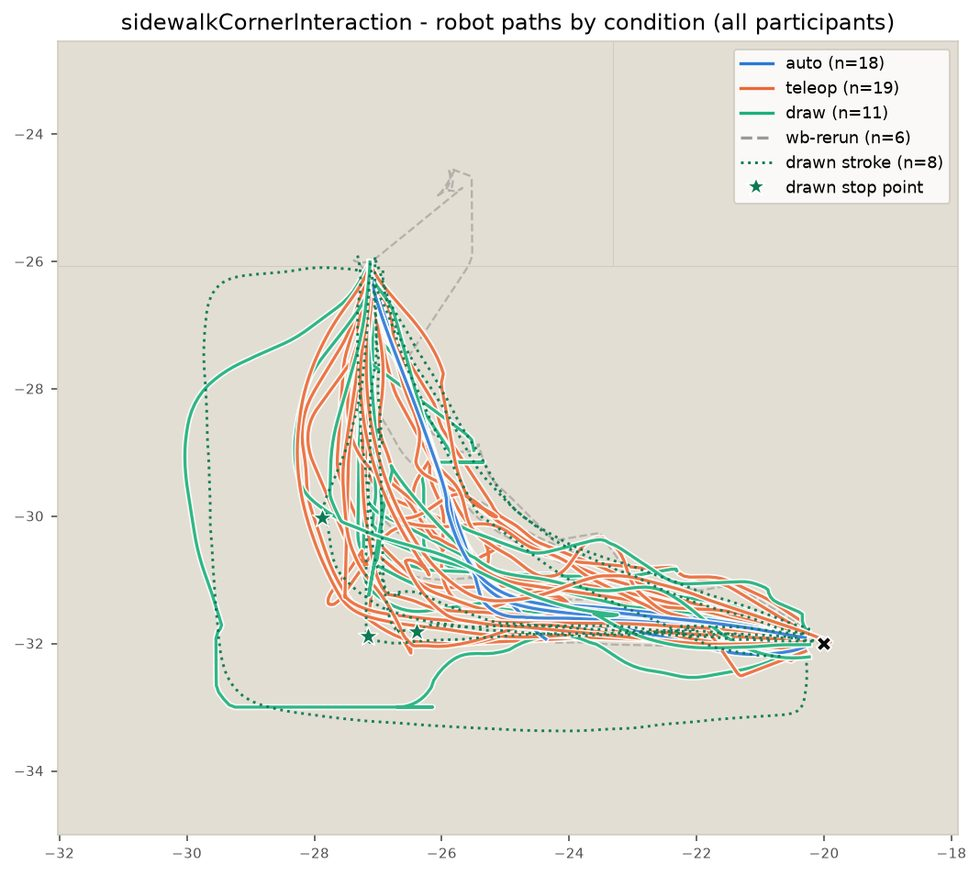
\includegraphics[width=\columnwidth]{figures_p1p13/fig_corner_p1p13.jpg}
  \caption{Corner interaction, all robot runs at P1--P13. The planner
  (blue) takes the tight inside line; driven paths (orange) fan wider;
  the drawn ideals (green, dotted) swing to the outer perimeter and
  carry explicit stop points ($\star$) --- the wide-arc doctrine
  rendered as geometry through the redraw tool.}
  \label{fig:corner}
\end{figure}

\textbf{At the blind corner the trade-off is efficiency against mutual
visibility, and visibility wins.} P5 took the efficient shortcut, then
recanted unprompted --- ``you never know if a person's around the
corner\dots\ socially it would have been more acceptable to swing out
wider into the middle, then turn once you know it's clear.'' P8 drove
the arc deliberately (``larger curvature so the human can see me --- if
I go close to the corner, it takes him by surprise'') and filed it as
the sanctioned exception to his own keep-right rule. P10 rejected the
inside line even where keep-right favoured it (``you're not gonna see a
person until the last minute''). P11 split the turn into two straight
legs with a pivot in place, so that every segment stays extrapolatable.

\textbf{At the head-on encounter the reasoning shifts from path shape
to stop placement: where you stop is the message.} Out of the flow but
still facing the person (P3); on stable ground rather than the grate
(P4, P5); out of the door-swing arc (P9: ``no point being out of the
way, only to be getting hit by doors''); all of it wrapped in P13's
motion policy --- ``go straight, but go slowly\dots\ set the right
expectation that I won't move wildly, and leave more room for the
pedestrian.''

\textbf{The redraw is the cleanest statement of preference we collect,
and the telemetry moves monotonically along it}
(Table~\ref{tab:ladder}). The planner never stops for anyone: 0.00
stops of at least one second near a human across all 74 autonomous
runs. Participants stop routinely, and the routes they \emph{drew}
stop longer still, slow down more near people, and give away more
efficiency than the routes they managed to drive. Spatially, the driven
paths agree with the planner only where nothing social happens ---
mean deviation 0.39\,m and Fr\'{e}chet distance 1.19\,m at the median
trial, with only 67\% of a typical human-driven path lying within half
a metre of the planner's line --- and the disagreement concentrates at
encounters (Figures~\ref{fig:corner} and~\ref{fig:narrow}).

\textbf{Three norms recur, with reasons attached.} \emph{Follow
people} --- a walker is a path-clearer, an oracle and a shield: P8,
``the human makes smarter decisions --- trail it, copy what it does'';
P9, ``they're already clearing a path\dots\ it's easier to follow in
someone's footsteps''; P11, at the crossing, ``if the person goes, I
follow them --- the driver can see a person and won't dare hit them.''
\emph{Do not match human walking speed} --- P7: ``it should either be
so fast that I don't have to wait for it, or so slow that I can bypass
it''; matched speed is the side-by-side trap the narrow-road telemetry
shows. \emph{Wait, but with a cap, then escalate} --- P13 imposed the
bound on herself mid-drive (``it would be unrealistic that I just keep
waiting\dots\ there should probably be a cap waiting time''), and P8
supplied the ladder: ``wait a couple seconds, signal; if nothing
happens, take the other route.''

\textbf{Strategies changed live inside the simulation}, which is the
concrete benefit of an interactive instrument over an interview. P3's
yielding policy rewrote itself the moment he learned the hatch could
trap his wheels (``I could theoretically get stuck in that\dots\ then
I'd wait for the person to pass me''); P8 converted terrain doubt
directly into deference (``I just waited for the human''); P5, boxed in
by the edited clutter, learned passability by watching the sim-human
thread the cones and then copied the route; P10, after blocking the
wide side of his own corner, produced the study's clearest courtesy
gesture --- a step back to cede the lane, ``a gesture that says: go
first.''

\textbf{Signalling proposals converge on a structure, not on a
modality.} Participants routed the modality by geometry and noise (P8:
visual when in the person's field of view, sound when behind them; P12:
voice where it is quiet, light where it is loud, anchored to the car
schema --- ``how we predict a car is to see the lights''); gated
announcements by proximity, density or a failed wait (P12: ``if the
human is within a certain distance, then say something --- not all the
time''; P10's wait-then-ring; P7's density-triggered alert); and asked
that the yield itself be made legible. P12's ``I'm waiting for you''
doubles as proof of detection (``then it's super clear I can just
go\dots\ oh, thank you! This robot is so smart!''); P10 demands a stop
that does not read as a breakdown (``not done, taking a break, or its
battery is dead''); P13 adds sequencing (``say excuse me, then wait one
or two seconds, for the pedestrian to be aware'').

\textbf{Every signal design presumes compliance, attribution and
ability --- three failure surfaces.} A signal is a contract that needs
a counterparty (P8: ``indicators would work, but if people don't adhere
to it, what's the point?''); with multiple robots the signal loses
attribution (P10: ``humans can't distinguish which one is giving the
signal''); and it must reach every body --- deaf pedestrians need the
visual channel, blind pedestrians the audio one, and P9 flags that
service animals are not trained on robots at all. Politeness fractures
the same way: ``excuse me'' is rude presumption to P2 (``it doesn't
mean I want to excuse you'') and P4 (``a human might be upset if a
robot tried to assume more importance than the human''), yet perfectly
welcome to P12 and P13. Voice splits identically --- ``creepy'' (P2),
``weird if it actually talked'' (P10), yet delight on the receiving end
when role-played (P12: ``oh! The robot is talking!'') --- with P4's
synthesis: ``a robot voice, but a kind robot voice.''

\textbf{Three disagreements stayed split, and read as personalisation
axes rather than design defects}: whether the robot should travel in
front or behind (P4 and P11 want it behind --- ``I can just forget
about it'' --- while P6, P8 and P9 want it visible in front --- ``I
don't trust it enough when I can't see it''); what to do about the
right-turning car (P5: the robot inherits pedestrian right-of-way and
should go; P4 and P13: wait, because right-of-way doesn't stop a
bumper; P11: it depends on whether local drivers actually yield --- a
fact about the country, not the robot); and the dedicated robot lane
(P2, P6 and P13 reach for infrastructure; P7 calls it premature and a
theft of bus-and-bike space; P8 notes it merely relocates the conflict
to every crossing).

% ---------------------------------------------------------------------
\subsection{Which scenarios participants find interesting or
concerning}
\label{sec:study:rq3}

\begin{figure}[t]
  \centering
  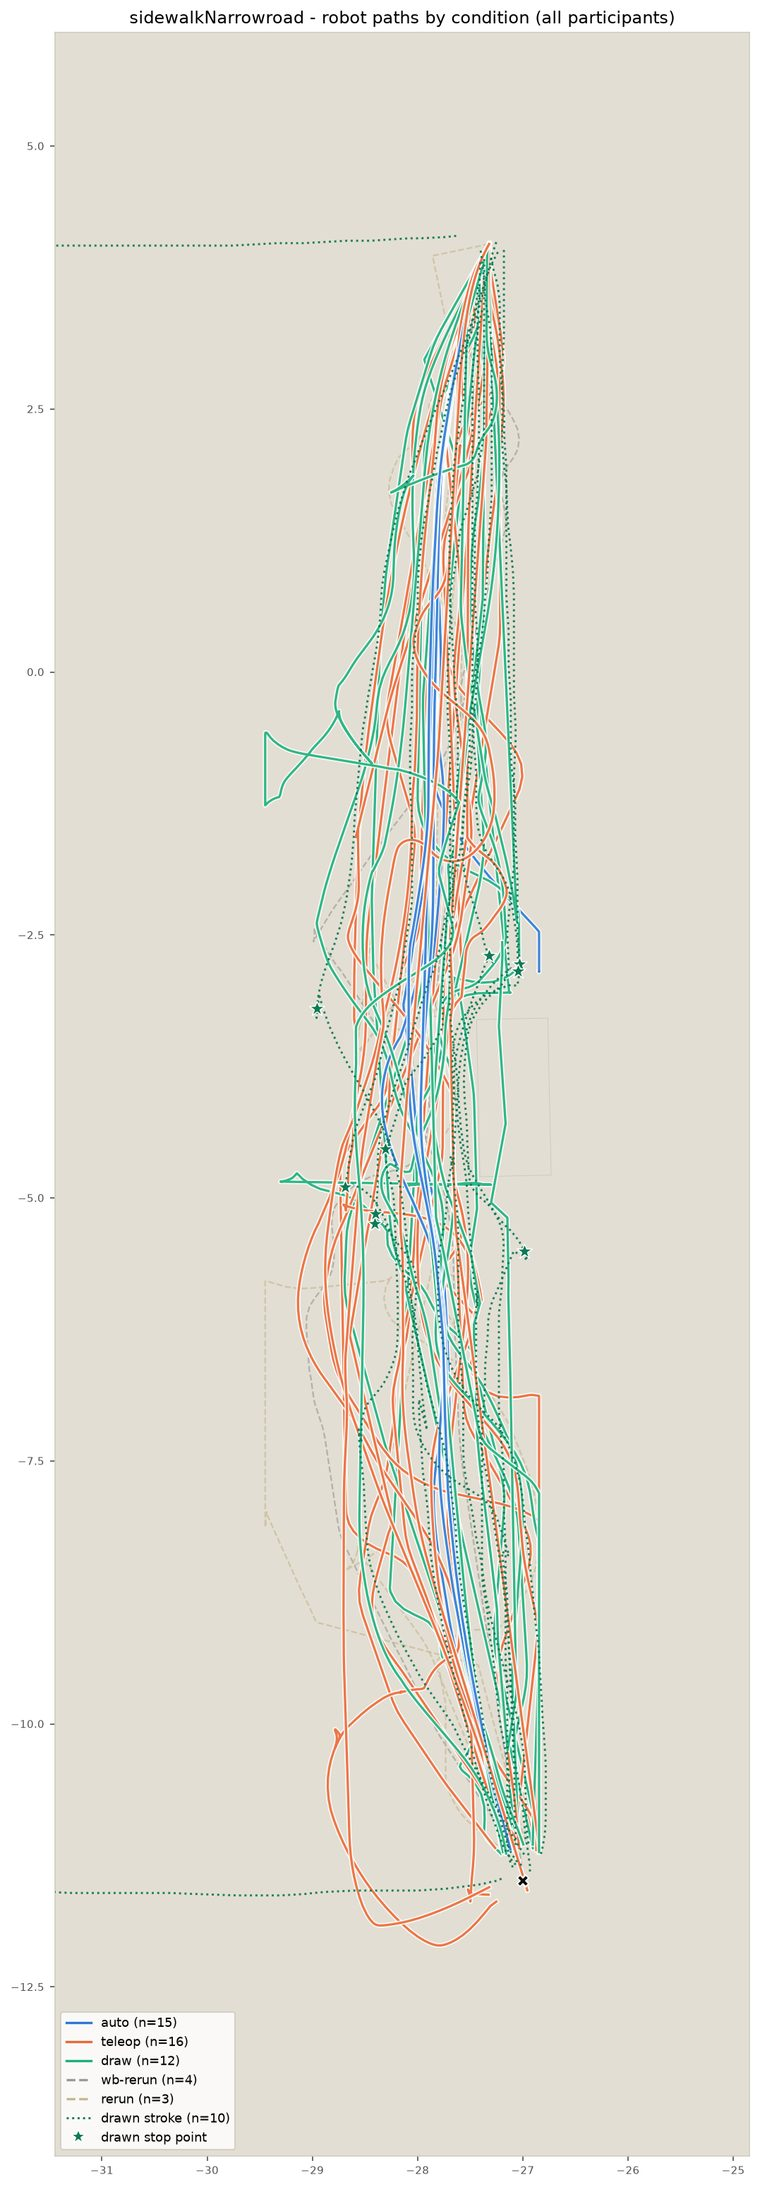
\includegraphics[width=\columnwidth]{figures_p1p13/fig_narrowroad_p1p13.jpg}
  \caption{Narrow road, all robot runs at P1--P13. The planner (blue)
  holds the centre line the whole way; driven (orange) and drawn
  (green) paths pull to the edges and scatter stop points ($\star$)
  along the margins --- ``pull aside, stop on stable ground, face the
  person'' enacted through the controller and the pen, not merely
  described.}
  \label{fig:narrow}
\end{figure}

\begin{table}[t]
  \centering
  \small
  \setlength{\tabcolsep}{4pt}
  \caption{What participants built when asked to make each scene
  harder: 143 objects across 39 edited worlds (P1--P13).}
  \label{tab:worlds}
  \begin{tabular}{lrr}
    \toprule
    \textbf{Scene} & \textbf{Objects} & \textbf{Character}\\
    \midrule
    Narrow road    & 50 & bottleneck clutter\\
    Corner         & 43 & occluders and approach traffic\\
    Out of store   & 31 & almost purely social (25/31 people)\\
    Crossroad      & 19 & geometry and behaviour edits instead\\
    \midrule
    \textbf{Total} & \textbf{143} & 58\% people or wheeled users\\
    \bottomrule
  \end{tabular}
\end{table}

The world-building phase turns concern into construction: given a
palette of people, wheeled users, props and ground conditions,
participants built the scenarios they believe matter. Across thirteen
participants they placed 143 objects across 39 edited worlds
(Table~\ref{tab:worlds}). \textbf{58\% of everything placed is a person
or a wheeled user} (83 of 143) --- participants build social pressure,
not obstacle courses. \textbf{83\% of the people they placed are
static}, which participants then discovered tests nothing social.
Sixteen mobility-aid users were placed by roughly half the panel,
unprompted: six wheelchairs, six mobility scooters and four cane users.

\textbf{The builds have per-scene signatures that go well beyond
``adding more people.''} The narrow road drew the heaviest
construction because its logic is the bottleneck --- P2, while
building: ``put something right opposite the table, where there's only
space for one person, and we get there at the same time --- like, what
are we gonna do?'' Out of store is almost purely social: 25 of its 31
placements are people, including the doorway-blocking chat groups of P5
(``sometimes people just talk in front of the restaurant\dots\ you'd
have to navigate around them''). The crossroad received the fewest
additions but the most edits to geometry and behaviour.

\textbf{Most builds were memories, not inventions.} P11 reconstructed
NYC scaffolding whose pole rows ``the robot can pass under but a person
can't,'' and split the puddle from the pothole --- one unpleasant, one
impassable. P9 placed cones because they get kicked: ``how do you get a
robot to navigate around something that's in the wrong spot?'' P10
recreated the reported Pittsburgh case of a robot camped on a curb cut
while a wheelchair user's crossing timer ran out. P13 assembled a
wheels-versus-feet ensemble --- a wheelchair user placed mid-path (``if
I were him, I'll take the middle --- less blockers''), a badly parked
scooter she confessed to parking herself, and a kid ``too short to get
noticed'' --- then asked for the mother-with-stroller the palette
lacked. P6 requested the study's only weather edit (rain, ``because it
can be hard to see the robot''). World building functioned as
elicitation of real deployment experience.

\textbf{Re-behaving the scene's agents formed a second axis of world
building, and produced several of the study's strongest probes}: the
erratic mirror-walker who paced the robot step for step (P7 read her
instantly as ``how an old person would react,'' and the
normal-behaviour re-run ``felt normal'' by contrast); the pedestrian
who never yields, which forced P11's robot into a dead stop and
generalised into his deadlock argument; speed swaps in both directions
(P9, slower than the robot: ``a leisurely pace --- I'm okay with it'';
P13 designing her own collision course --- ``maybe I walk slower so I
can run into a robot?''); and the forced-straight control that deleted
the problem entirely (P3). Together with the object edits these form
paired manipulations --- erratic\,$\leftrightarrow$\,predictable,
yielding\,$\leftrightarrow$\,non-yielding,
faster\,$\leftrightarrow$\,slower --- which is what licenses
\S\ref{sec:study:rq1}'s separation of predictability from proximity.

\textbf{Three concerns recur that no navigation policy addresses
alone.} \emph{Cars that cannot see a knee-high robot}, raised
independently by eight participants, with a shared mitigation ---
cross behind a human the driver can see. \emph{Harassment and theft},
including the four-times-replicated urgency-disclosure dilemma:
announcing ``medicine on board'' negotiates priority and invites
robbery in the same breath (P2, P3, P4, P8). And \emph{density
ceilings} --- P11's Berkeley convoy jam as the observed end state,
with P7's geographic irony that robots are most useful exactly where
density defeats them.

Two notes fall directly out of the builds for the simulator itself.
Static added humans become furniture --- P4 ``treated them as regular
obstacles to go around, instead of having behavior to consider,'' and
P7 agrees (``objects are easy --- you don't have to predict their
behavior'') --- so social world building needs moving agents by
default. And behaviour-level editing (speed, yielding, erraticness)
proved as analytically productive as object placement, so it deserves
first-class interface support rather than wizard improvisation.

% ---------------------------------------------------------------------
\subsection{Threats to validity}
\label{sec:study:limits}

\textbf{The blind corner is not blind.} Both goal markers are labelled
and visible throughout, so neither agent is ever genuinely uncertain
about the other's destination, and participants said so unprompted:
``Because I knew there was a robot, I stayed to the edge --- and on a
normal day I probably would have walked in the center'' (P2). Since the
central finding of \S\ref{sec:study:rq1} concerns uncertainty about
intent, goal visibility should become a manipulated variable rather
than a constant.

\textbf{The human-side comparison is confounded by which agent the
participant embodies.} The wheelchair agent is driven by the
participant in autonomous-robot trials but falls to the scripted
social-force controller once the participant moves into the robot. Any
auto-versus-manual contrast computed on wheelchair-side measures
therefore compares a human-driven wheelchair against a scripted one and
cannot be read as an effect of the robot's controller. We consequently
report no human-disruption contrast, and proximity measures are joint
outcomes of both agents.

\textbf{Teleoperation confounds skill with intent.} Close-approach and
personal-space counts under joystick control partly reflect controller
proficiency rather than social intent; the drawn condition is the
cleaner statement of preference, and Table~\ref{tab:ladder} should be
read with that asymmetry in mind.

\textbf{Flat ground makes surface conditions invisible.} Participants
ignored the ground until a researcher pointed at it, because nothing in
the simulation punishes them for it --- ``just because it's a game, I'm
not seeing the robot jiggle as I move it. So in my head, that's a
smooth one'' (P3). Given that infrastructure was among the
first-named deployment challenges, the absence of terrain feedback is a
substantive gap rather than a fidelity nicety.

\textbf{Instrumentation.} The background pedestrian follows fixed
waypoint routes and does not react, so it should not be treated as a
second social agent. Scenario order varied between participants, so
scenario-level ratings are ordinal. The world-editor's scene-delta
recorder logs any object displaced from its baseline regardless of
cause, so object \emph{relocations} are not reported here as a
participant behaviour: the majority of recorded displacements are
artefacts of a scripted vehicle that drives during the preceding trial
in the same loaded scene. Placements, which cannot be produced this
way, are the reliable world-building measure. Finally, the VLM capture
and signal-annotation channels are empty across all trials, so no
finding here speaks to the robot's perception, or to signalling as
implemented --- only to signalling as participants imagined it.
